%!TEX program = xelatex

\documentclass[compress]{beamer}
%--------------------------------------------------------------------------
% Common packages
%--------------------------------------------------------------------------
\usepackage[english]{babel}
\usepackage{pgfpages} % required for notes on second screen
\usepackage{graphicx}

\usepackage{multicol}

\usepackage{tabularx,ragged2e}
\usepackage{booktabs}

% fancy source code
% !! require calling latex with -shell-escape !!
\usepackage[cache]{minted}
\renewcommand{\theFancyVerbLine}{
  \sffamily\textcolor[rgb]{0.5,0.5,0.5}{\scriptsize\arabic{FancyVerbLine}}}

\newminted{python}{frame=lines,
                    linenos=true,
                    gobble=4,
                    fontsize=\scriptsize,
                    xleftmargin=1.8em}

%--------------------------------------------------------------------------
% Load theme
%--------------------------------------------------------------------------
\usetheme{hri}

\usepackage{dtklogos} % must be loaded after theme
\usepackage{tikz}
\usetikzlibrary{mindmap,backgrounds,positioning}

\graphicspath{{figs/}}

%--------------------------------------------------------------------------
% General presentation settings
%--------------------------------------------------------------------------
\title{MORSE \& HRI}
\subtitle{Recent Perspectives}
\date{\today}
\author{Séverin Lemaignan, Marc Hanheide, \\ Michael Karg, Harmish Khambhaita,
\\Lars Kunze, \underline{Florian Lier}, \\Ingo Lütkebohle and Grégoire Milliez}

%--------------------------------------------------------------------------
% Notes settings
%--------------------------------------------------------------------------
%\setbeameroption{show notes on second screen}

\begin{document}

\maketitle

%--------------------------------------------------------------------------
% Table of contents
%--------------------------------------------------------------------------

\section*{Overview}
\begin{frame}{Overview}
    % hideallsubsections ist empfehlenswert für längere Präsentationen
    \tableofcontents[hideallsubsections]
\end{frame}

%%%%%%%%%%%%%%%%%%%%%%%%%%%%%%%%%%%%%%%%%%%%%%%%%%%%%%%%%%%%%%%%%%%%%%%%%%%%%%
%%%%%%%%%%%%%%%%%%%%%%%%%%%%%%%%%%%%%%%%%%%%%%%%%%%%%%%%%%%%%%%%%%%%%%%%%%%%%%
%%%%%%%%%%%%%%%%%%%%%%%%%%%%%%%%%%%%%%%%%%%%%%%%%%%%%%%%%%%%%%%%%%%%%%%%%%%%%%

\section{Brief Recap of MORSE}


\begin{frame}{A "Software in the Loop" simulator}
    \begin{figure}
        \centering
        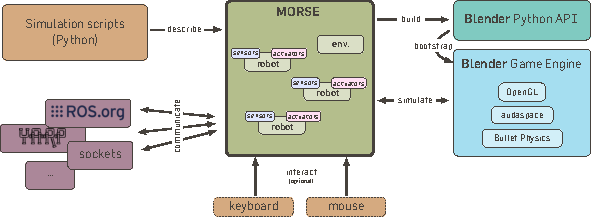
\includegraphics[width=\linewidth]{morse}
    \end{figure}
\end{frame}

\begin{frame}{Levels of abstraction}
    \begin{figure}
        \centering
        \includegraphics<1>[width=\linewidth]{realism-0}
        \includegraphics<2>[width=\linewidth]{realism-1}
        \includegraphics<3>[width=\linewidth]{realism-2}
        \includegraphics<4>[width=\linewidth]{realism-3}
    \end{figure}
\end{frame}


\begin{frame}[fragile]
    \begin{multicols}{2}
        \null \vfill
\begin{pythoncode}
    from random import uniform
    from morse.builder import *

    robot = PR2()

    for h in range(30):
        human = Human()
        human.translate(
                uniform(-5, 5), 
                uniform(-5, 5), 
                0)

        human.rotate(
                0, 
                0, 
                uniform(0, 360))

    env = Environment('sandbox')
\end{pythoncode}

        \vfill \null
        \columnbreak
        \null \vfill
        \begin{figure}
            \centering
            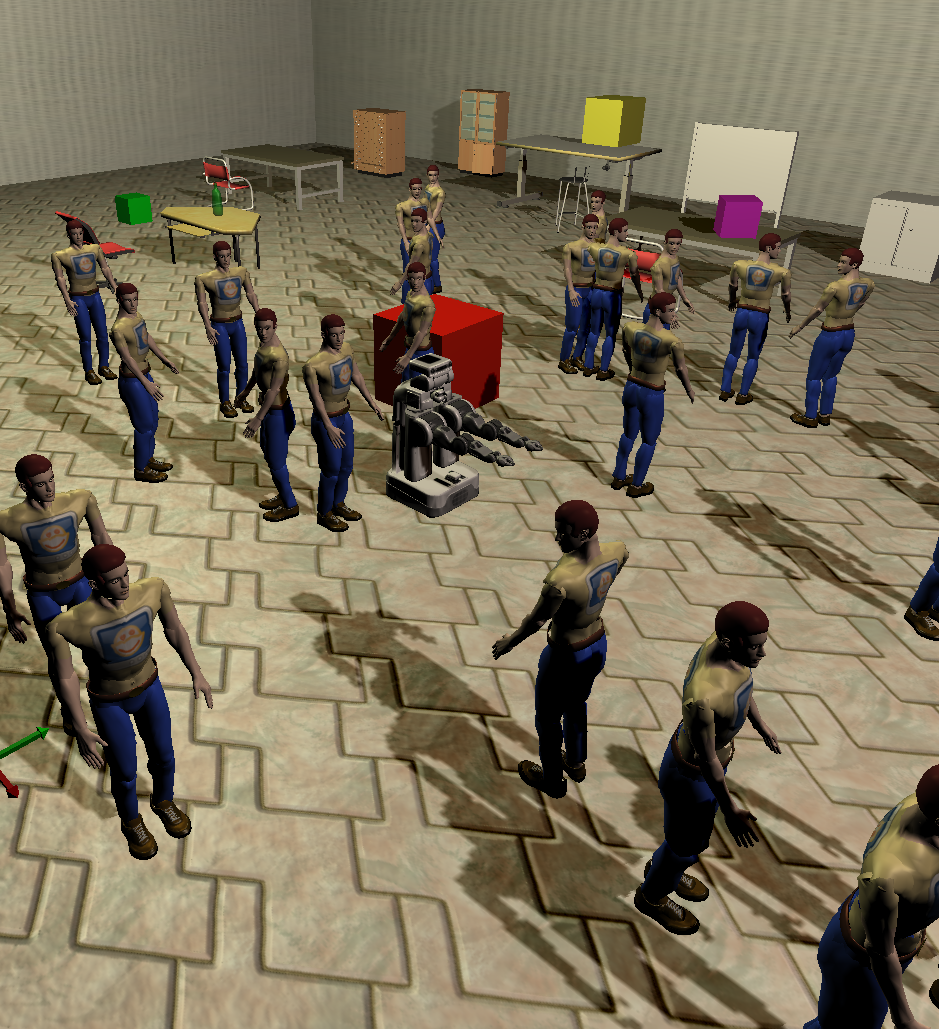
\includegraphics[width=\linewidth]{30humans}
        \end{figure}
        \vfill \null
    \end{multicols}
\end{frame}

\imageframe[Not there yet...]{morse-hri}


%%%%%%%%%%%%%%%%%%%%%%%%%%%%%%%%%%%%%%%%%%%%%%%%%%%%%%%%%%%%%%%%%%%%%%%%%%%%
%%%%%%%%%%%%%%%%%%%%%%%%%%%%%%%%%%%%%%%%%%%%%%%%%%%%%%%%%%%%%%%%%%%%%%%%%%%%
%%%%%%%%%%%%%%%%%%%%%%%%%%%%%%%%%%%%%%%%%%%%%%%%%%%%%%%%%%%%%%%%%%%%%%%%%%%%

\section{Simulating HRI}

\begin{frame}{Situation Assessment with Human}
    \begin{figure}
        \centering
        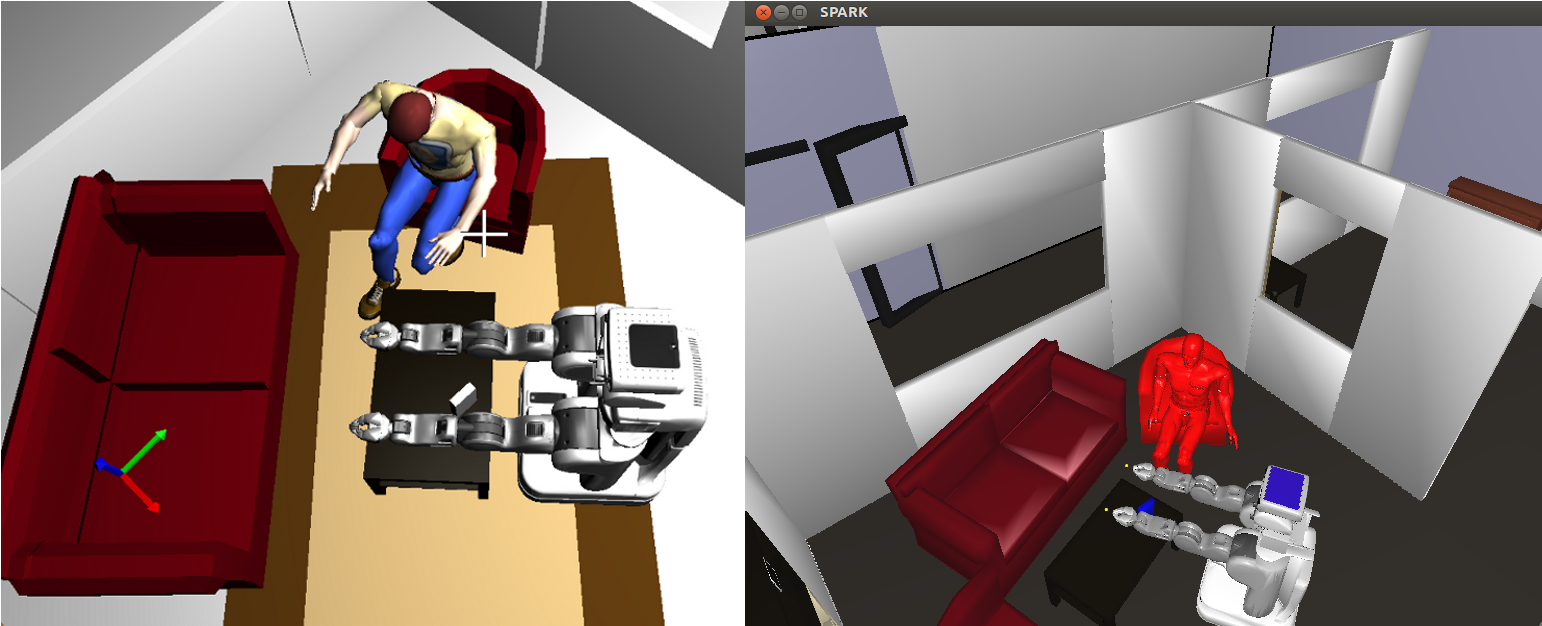
\includegraphics[width=\linewidth]{morsespark}
    \end{figure}
\end{frame}

\begin{frame}{Large Scenarii}
    \begin{figure}
        \centering
        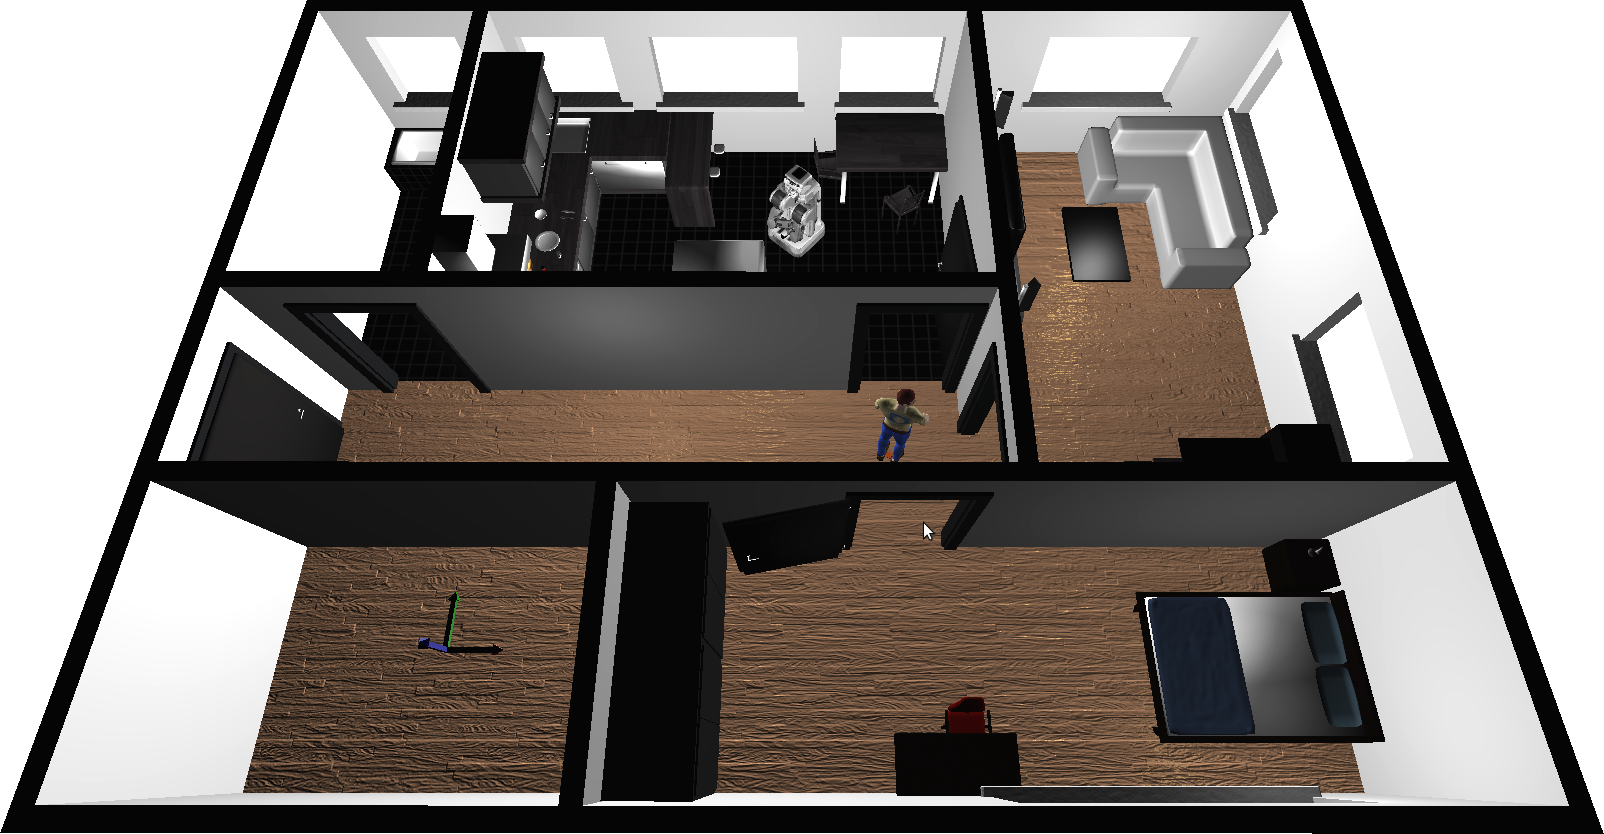
\includegraphics[width=\linewidth]{morse_apartment}
    \end{figure}
\end{frame}

\begin{frame}{Refining Algorithms}
    \begin{multicols}{2}
        \null \vfill
    \begin{figure}
        \centering
        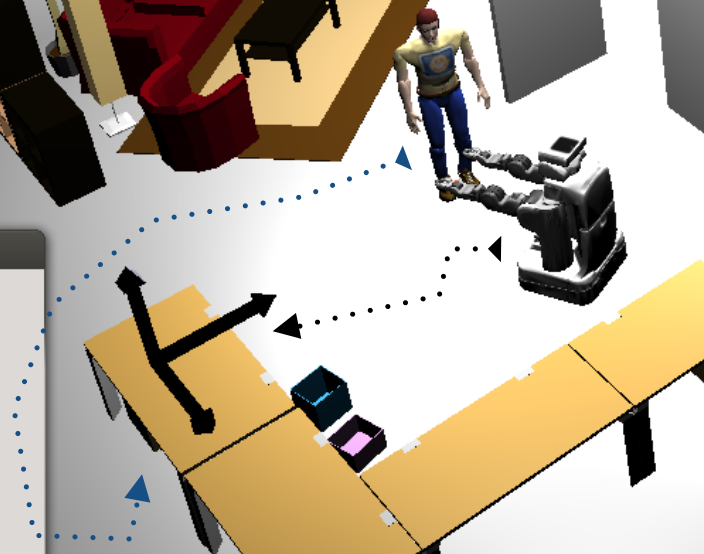
\includegraphics[width=0.9\linewidth]{proto-setup}
    \end{figure}

        \vfill \null
        \columnbreak
        \null \vfill
        \begin{figure}
            \centering
            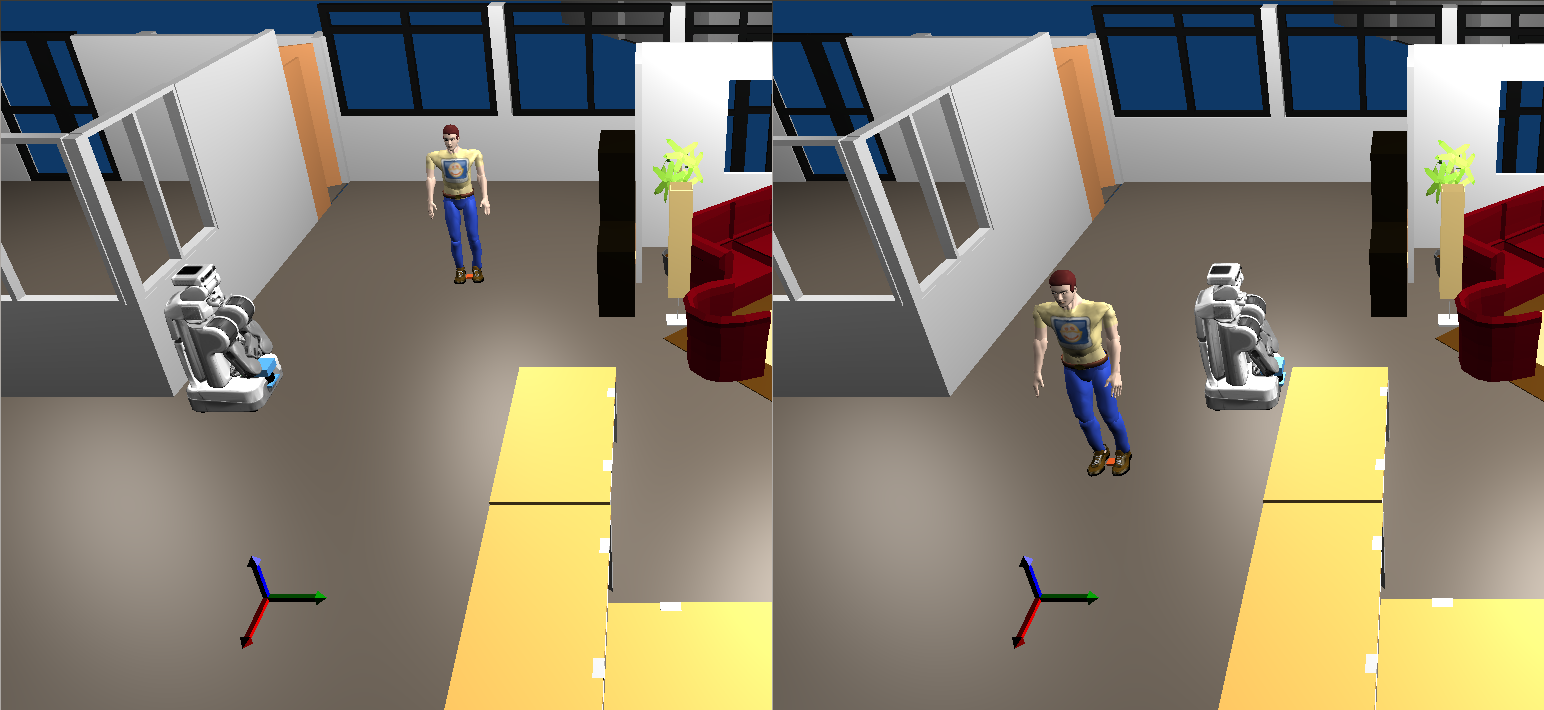
\includegraphics[width=0.9\linewidth]{morsehanp}
        \end{figure}
        \vfill \null
    \end{multicols}
\end{frame}

\begin{frame}{Benefits}
    \begin{itemize}
        \item Repeatable: fine for benchmarks, regression tests,
        \item Abstraction levels: simulate only what is needed,
        \item \emph{Computer game}-style, tests can be carried by one researcher
            alone: support iterative design and implementation,

    \end{itemize}
\end{frame}


\section{Less Usual Use-cases}

\begin{frame}{Automatic Human-like Scene Generation}
    \begin{figure}
        \centering
        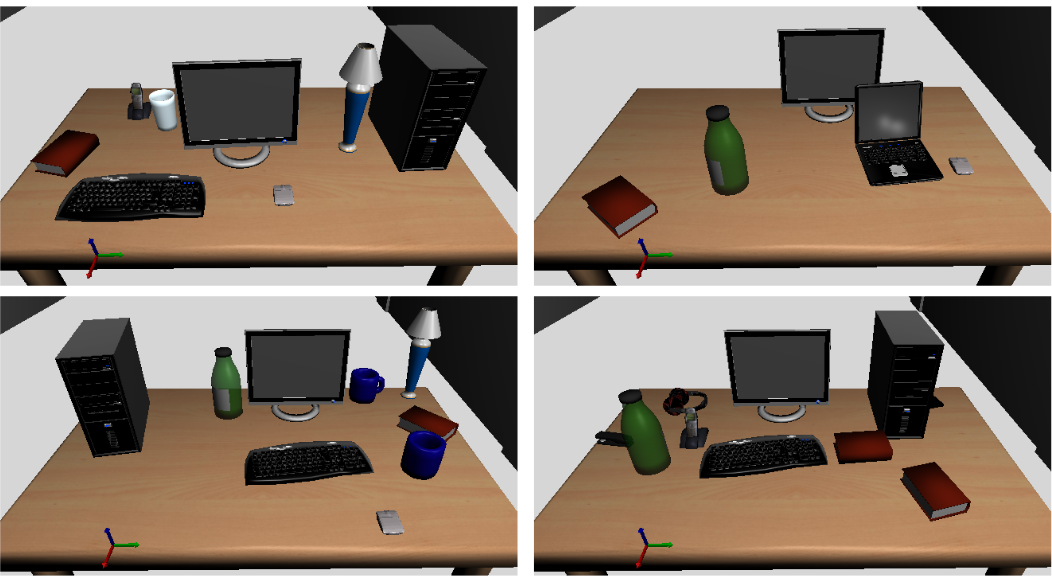
\includegraphics[width=\linewidth]{scenes}
    \end{figure}
\end{frame}


\begin{frame}{Continuous Integration and HRI}
    \begin{figure}
        \centering
        %\includegraphics[width=\linewidth]{}
    \end{figure}
\end{frame}


\section{What Next?}

\imageframe[Soon there?]{morse-hri}

\begin{frame}{MakeHuman Integration}
    \begin{figure}
        \centering
        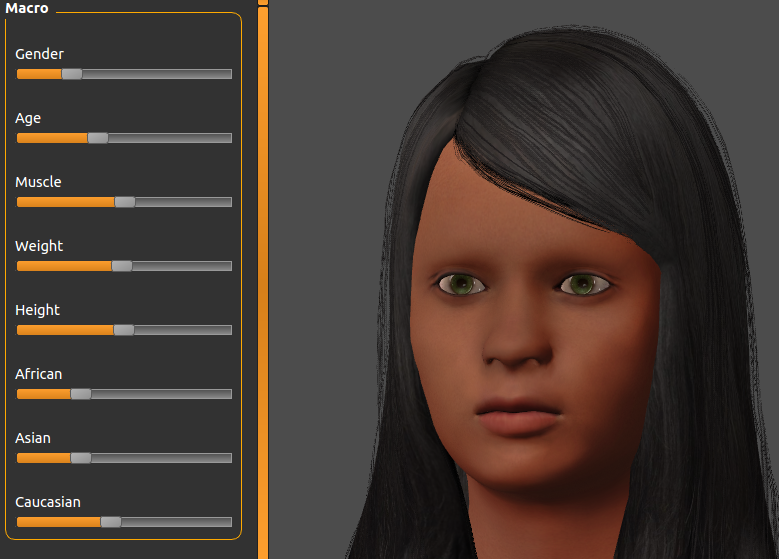
\includegraphics[width=\linewidth]{makehuman}
    \end{figure}
\end{frame}


\begin{frame}{What Next?}
    \begin{itemize}
        \item<1-> Autonomous navigation of humans
        \item<2-> Crowd simulation
        \item<3-> Better library of motions (walk cycles, pick/place, emotions...)
    \end{itemize}

    \uncover<4->{
    Open "HRI" issues on GitHub: \url{https://github.com/morse-simulator/morse/labels/HRI}
}
\end{frame}


\maketitle

\end{document}






